\documentclass[12pt,a4paper]{report}
\usepackage[utf8]{inputenc}
\usepackage{amsmath}
\usepackage{amsfonts}
\usepackage{amssymb}
\usepackage{graphicx}
\author{Frederik Appel Vardinghus-Nielsen}
\begin{document}
\noindent{\Huge Optimization methods}\\\\
\textbf{Preparation:}
\begin{itemize}
\setlength\itemsep{0em}
\item[-] The student blindly draws one topic from the pool of the eight different topics described above.
\item[-] The student then has 15 minutes preparation time before the exam.
\item[-] Notice that this preparation is open book - all study material is allowed in the preparation room .
\end{itemize}
\textbf{Exam:}
\begin{itemize}
\setlength\itemsep{0em}
\item[-] First, the examiner will ask a couple of questions on the miniproject.
\item[-] Then, the examiner will ask a couple of questions on the topic that was drawn.
\item[-] We expect that the discussion will take place at the blackboard.
\item[-] During the exam books/slides are not allowed but you may bring your own notes.
\item[-] It is not expected that you can do all the intermediate derivations of the theory/algorithms.
\item[-] It is expected that you understand the conditions and can interpret the results of the theory/algorithms covered in this course.
\item[-] The total time for the oral examination (excluding preparation time) is about 15 - 20 minutes including evaluation.
\end{itemize}
\textbf{Topics:}
\begin{itemize}
\setlength\itemsep{0em}
\item[] Constrained Optimization
\item[] Linear Programming and The Simplex Method
\item[] Duality and Iterative Methods
\item[] Interpoint methods
\item[] Alternating Direction Methods of Multipliers (ADMM)
\item[] Semidefinite Relaxation
\item[] Simulated Annealing
\item[] Genetic algorithms
\end{itemize}
\clearpage
\noindent{\Huge Constrained Optimization}\\\\
Chapter 10 covers most of this subject.
\\\\
\textbf{First-Order Necessary Conditions for a Minimum}
\begin{itemize}
\item[(a)] If $f(x)\in C^1$ and $x^*$ is a local minimizer, then
\begin{equation}
g(x^*)^T d \geq 0
\end{equation}
for every feasible direction $d$ at $x^*$.
\item[(b)] If $x^*$ is located in the interior of $\mathbf{R}$, then
\begin{equation}
g(x^*)=0
\end{equation}
\end{itemize}
\textbf{Second-Order Necessary Conditions for a Minimum}
\begin{itemize}
\item[(a)] If $f(x)\in C^2$ and $x^*$ is a local minimizer, then for every feasible direction $d$ a $x^*$
\begin{itemize}
\item[(i)] $g(x^*)^Td \geq 0$
\item[(ii)] If $g(x^*)^Td=0$, then $d^TH(x^*)d\geq0$
\end{itemize}
\item[(b)] If $x^*$ is a local minimizer in the interior of $\mathcal{R}$, then
\begin{itemize}
\item[(i)] $g(x^*)=0$
\item[(ii)] $d^TH(x^*)d\geq0$ for all $d\neq0$
\end{itemize}
\end{itemize}
\textbf{Second-Order Sufficient Conditions for a Minimum}\\
If $f(x)\in C^2$ and $x^*$ is located in the interior of $\mathcal{R}$, then the conditions
\begin{itemize}
\item[(a)] $g(x^*)=0$
\item[(b)] $H(x^*)$ is positive semi definite
\end{itemize}
are sufficient for $x^*$ to be a strong local minimizer.
\\\\
\textbf{See section 10.3, page 273 for classification of constrained optimization problems.}
\begin{itemize}
\setlength\itemsep{0em}
\item Linear programmming
\item Quadratic programmming
\item Convex programming
\item General constrained optimization problem
\end{itemize}
Consider the problem of nonlinear equality constraints and variable transformations.
\\\\
\textbf{Lagrange multipliers}\\
At a local minimizer of a constrained optimization problem, the gradient of the objective function is a linear combination of the gradients of the constraints.
\begin{equation}
\nabla f(x^*)=\sum_{i=1}^p\lambda_i^*\nabla a_i(x^*)
\end{equation}
\textbf{First-Order Necessary Conditions for a Minimum, Equality Constraints}\\
If $x^*$ is a constrained minimizer of an equality contrained problem and is a regular point of the contraints, then
\begin{itemize}
\item[(a)] $a_i(x^*)=0$ for $i=1,2,\ldots,p$
\item[(b)] There exist Lagrange multipliers $\lambda_i^*$ for $i=1,2,\ldots,p$ such that
\begin{equation}
\nabla f(x^*)=\sum_{i=1}^p\lambda_i^*\nabla a_i(x^*)
\end{equation}
\end{itemize}
\textbf{First-Order Necessary Conditions for a Minimum, Inequality Constraints}\\
If $x^*$ is a constrained minimizer of an inequality constrained problem and is a regular point of the constraints, then
\begin{equation}
\nabla f(x^*)=\sum_{i=1}^p\lambda_i^*\nabla a_i(x^*)+\sum_{k=1}^K\mu_{j_k}^*\nabla c_{j_k}(c^*)
\end{equation}
where $K$ is the number of active inequality constraints.\\\\
\textbf{Karush-Kuhn-Tucker conditions}\\
Build upon Lagrange multipliers for constrained problems. See theorem 10.2, page 298 in Practical Optimization for full theorem.\\\\
\textbf{Second-Order Necessary Conditions for a Minimum, Equality Constraints}\\
See theorem 10.3, page 303, and forward.\\\\
\textbf{Necessary and Sufficient Conditions for a Minimum in Alternative-Form LP Problem}\\
See theorem 11.1 on page 325.
\clearpage

\noindent{\Huge Linear Programming and the Simplex Method}\\\\
\textbf{LP Standard Form}
\begin{align*}
\text{minimize }f(x)&=c^Tx\\
\text{subject to: }Ax&=b\\
x&\geq0
\end{align*}
If the problem is on alternative form it can reformulated by introducing slack variables.
\begin{align*}
Ax-y&=b&\text{for }y\geq0\\
x&=x^+-x^-&x^+\geq0\text{ and }x^-\geq0
\end{align*}
The problem then becomes
\begin{align*}
\hat{x}=\begin{bmatrix}x^+\\x^-\\y\end{bmatrix},&\hat{c}=\begin{bmatrix}c\\-c\\0\end{bmatrix},&\hat{A}=\begin{bmatrix}A&-A&-I_p\end{bmatrix}
\end{align*}
with
\begin{align*}
\text{minimize }f(x)&=\hat{c}^T\hat{x}\\
\text{subject to }\hat{A}\hat{x}&=b\\
\hat{x}&\geq0
\end{align*}
\textbf{KKT conditions are found in theorem 11.1 on page 324}\\\\
\textbf{Polytopes}\\
The feasible region defined by $\mathcal{R}=\{x:Ax\geq b\}$ is in general convex. A set of points $\mathcal{F}$ is said to be a face of $\mathcal{R}$ if $p_1,p_2\in\mathcal{F}\,\implies\,(p_1+p_2)/2\in\mathcal{F}$. If $l$ is the dimension of a face $\mathcal{F}$, a facet is an $(l-1)$-dimensional face, an edge is a one-dimensional face and a vertex is a zero dimensional face.\\\\
\textbf{See theorem 11.3 and 11.4 for sufficient and necessary conditions for minimum in LP problem.}\\\\
\textbf{Simplex Method}\\
See page 344 in Pract	ical Optimization.
\clearpage
\noindent{\Huge Duality and Iterative Methods}\\\\
\textbf{Jacobi method}\\
Solve a system of linear equations with the Jacobi method:
\begin{equation}
Ax=b
\end{equation}
Decompose $A=D+R$ where $D$ is diagonal. The solution $x$ is then obtained by
\begin{align*}
x^{(k+1)}&=D^{-1}(b-Rx^{(k)})\\
x_i^{(k+1)}&=\frac{1}{a_{ii}}\left(b_i-\sum_{j\neq i}a_{ij}x_k^{(k)}\right),&i=1,\ldots,n
\end{align*}
\textbf{Gauss-Seidel method}\\
Solves the system
\begin{equation}
Ax=b
\end{equation}
by decomposing $A$ into a lower triangular matrix $L_*$ and a strictly upper triangular matrix $U$:
\begin{equation}
L_*x=b-Ux
\end{equation}
The iterations are described by
\begin{align*}
x^{(k+1)}&=L_*^{-1}(b-Ux^{(k)}\\
x_i^{(k+1)}&=\frac{1}{a_{ii}}\left(b_i-\sum_{j=1}^{i-1}a_{ij}x_j^{(k+1)}-\sum_{j=i+1}^na_{ij}x_j^{(k)}\right),&i=1,\ldots,n
\end{align*}
\textbf{Lagrangian Dual Function}
Given problem
\begin{align*}
\text{minimize }&f_0(x)\\
\text{subject to }&f_i(x)\leq0,&i=1,\ldots,m\\
&h_i(x)=0,&i=1,\ldots,p
\end{align*}
Lagrangian function is defined as
\begin{equation}
\mathcal{L}(x,\lambda,\nu)=f_0(x)+\sum_{i=1}^m\lambda_if_i(x)+\sum_{i=1}^p\nu_ih_i(x)
\end{equation}
Lagrangian dual function defined as
\begin{equation}
g(\lambda,\nu)=\inf_{x\in \mathcal{D}}\mathcal{L}(x,\lambda,\nu)=\inf_{x\in \mathcal{D}}\left(f_0(x)+\sum_{i=1}^m\lambda_if_i(x)+\sum_{i=1}^p\nu_ih_i(x)\right)
\end{equation}
If $p^*$ is optimal value for original (primal) problem, then
\begin{equation}
g(\lambda,\nu)\leq p^*
\end{equation}
The Lagrange dual problem considers maximizing $g$ for some $\lambda \succeq 0$:
\begin{align*}
\text{maximize }&g(\lambda,\nu)\\
\text{subject to }&\lambda\succeq0
\end{align*}
Weak duality is when the solution to the Lagrange dual problem is less than the solution to the primal problem:
\begin{equation}
d^*\leq p^*
\end{equation}
Difference between $d^*$ and $p^*$ is called the optimal duality gap. If $d^*=p^*$ it is called strong duality.
\begin{itemize}
\item Exact line search
\begin{equation}
t=argmin_{s\geq0} f(x+s\Delta x)
\end{equation}
\item Backtracking line search: $0<\alpha<0.5$, $0<\beta<1$.
\begin{equation}
f(x+t\Delta x)>f(x)+\alpha t\nabla f(x)^T\Delta x,\phantom{mm}t:=\beta t
\end{equation}
\item Gradient descent method
\begin{equation}
\Delta x = -\nabla f(x)
\end{equation}
Stopping criterion:
\begin{equation}
\Vert \nabla f(x)\Vert_2
\end{equation}
\item Steepest descent\\
Use Taylor's:
\begin{equation}
f(x+v)\approx \hat{f}(x+v)=f(x)\nabla f(x)^Tv
\end{equation}
The second term is the directional derivative of $f$. The normalized steepest descent direction with respect to some norm $\Vert\cdot\Vert$ is defined as
\begin{equation}
\Delta x_{nsd}=argmin\{\nabla f(x)^Tv\,|\,\Vert v\Vert=1\}.
\end{equation}
Use backtracking line search for distance travelled along the descent.
\item Newton Step
\begin{equation}
\Delta x_{nt}=-\nabla^2f(x)^{-1}\nabla f(x)
\end{equation}
The Newton step is a descent or optimal from the fact of positive definiteness og the Hessian:
\begin{equation}
\nabla f(x)^T\Delta x_{nt}=-\nabla f(x)^T\nabla^2f(x)^{-1}\nabla f(x)<0
\end{equation}
Newton step is the steepest descent in the Hessian norm. The Newton step is optimal close to the minimizing point. Use
\begin{equation}
\lambda^2=\nabla f(x)^T\nabla^2f(x)^{-1}\nabla f(x)
\end{equation}
for quitting when $\lambda^2/2\leq\epsilon$. Use backtracking line search.
\end{itemize}
\clearpage
\noindent{\Huge Interior-Point Methods}\\\\
\textbf{Barrier method}\\
Used for a problem with inequality constraints:
\begin{align*}
\text{minimize }&f_0(x)\\
\text{subject to }&f_i(x)\leq0,&i=1,\ldots,m\\
&Ax=b
\end{align*}
Assume that the problem is strictly feasible meaning there exists $x\in\mathcal{D}$ such that $f_i(x)<0$ $\forall i$. With Slater's condition dual optimal $\lambda^*$ and $\nu^*$ exist and KKT conditions are fulfilled:
\begin{align*}
Ax^*=b,\phantom{mm}f_i(x^*)&\leq0,&i=1,\ldots m\\
\lambda^*&\succeq0\\
\nabla f_0(x^*)+\sum_{i=1}^m\lambda_i^*\nabla f_i(x^*)+A^T\nu^*&=0\\
\lambda_i^*f_i(x^*)&=0,&i=1,\ldots m
\end{align*}
Example:
\begin{align*}
\text{minimize }&f_0(x)+\sum_{i=1}^mI_-f_i(x))\\
\text{subject to }&Ax=b
\end{align*}
where $I_-(u)=0$ for $u\leq0$ and $I_-(u)=\infty$ otherwise. $I_-(u)$ is approximated by a logarithmic function:
\begin{equation}
\hat{I}_-(u)=-(1/t)\log(-u),\phantom{mm}\mathbf{dom}\hat{I}_-=-\mathbb{R}_{>0}
\end{equation}
Use Newton's method to solve.
where $t>0$ sets accuracy. $\hat{I}$ is convex, differentiable and increasing and therefore easier to handle. The central path is the path for $x$ towards the optimal value of the original problem, when $t\to\infty$. The problem described by
\begin{align*}
\text{minimize }&tf_0(x)+\phi(x)\\
\text{subject to }&Ax=b
\end{align*}
has central points $x^*(t)$ on the central path. $x^*(t)$ is found by
\begin{equation}
t\nabla f_0(x^*(t))+\sum_{i=1}^m\frac{1}{-f_i(x^*(t))}\nabla f_i(x^*(t))+A^T\hat{\nu}
\end{equation}
\textbf{Dual points and convergence}\\
Define
\begin{equation}
\lambda_i^*(t)=\frac{1}{tf_i(x^*(t))}\phantom{mm}\nu^*(t)=\hat{\nu}/t
\end{equation}
These are dual feasible points and therefore yield a lower bound from the dual function:
\begin{align*}
p^*=g(\lambda^*,\nu^*)&=f_0(x^*(t))+\sum_{i=1}^m\lambda_i^*(t)f_i(x^*(t))+\nu^*(t)^T(Ax^*(t)-b)\\
&=f_0(x^*(t))-m/t
\end{align*}
As such the duality gap is
\begin{equation}
f_0(x^*(t))-p^*=m/t
\end{equation}
\clearpage
\noindent{\Huge Alternating Direction Methods of Multipliers (ADMM)}\\\\
Solves problems of the form
\begin{align*}
\text{minimize }&f(x)+g(z)\\
\text{subject to }&Ax+Bz=c
\end{align*}
Utilizes the splitting of functions (dual ascent property) and superior convergence (method of multipliers). optimal value denoted by
\begin{equation}
p^*=\inf \{f(x)+g(z)|Ax+Bz=c\}
\end{equation}
Form augmented Lagrangian and update steps:
\begin{align*}
\mathcal{L}_{\rho}(x,z,y)&=f(x)+g(x)+y^T(Ax+Bz-c)+\frac{\rho}{2}\Vert Ax+Bz-c\Vert_2^2\\
x^{k+1}&=argmin\mathcal{L}_{\rho}(x,z^k,y^k)\\
z^{k+1}&=argmin\mathcal{L}_{\rho}(x^{k+1},z,y^k)\\
y^{k+1}&=y^k+\rho(Ax^{k+1}+Bz^{k+1}-c)
\end{align*}
\textbf{Convergence}
\begin{itemize}
\item \textit{Residual Convergence}: $r^k\to0$ as $k\to\infty$
\item \textit{Objective convergence}: $f(x^k)+g(z^k)\to p^*$ as $k\to\infty$
\item \textit{Dual variable convergence}: $y^k\to y^*$ as $k\to\infty$
\end{itemize}
\textbf{Optimality conditions}
Necessary and sufficient conditions include primal feasibility
\begin{equation}
Ax^*+Bz^*-c=0
\end{equation}
and dual feasibility
\begin{align*}
0&\in\partial f(x^*)+A^Ty^*\\
0&\in\partial g(x^*)+B^Ty^*
\end{align*}
\textbf{Stopping criteria}
\begin{align*}
\Vert r^k\Vert_2&=\Vert Ax+Bz-c\Vert_2\leq \epsilon^{pri}\\
\Vert s^k\Vert_2&=\Vert\rho A^TB(z^{k+1}-z^k)\Vert_2\leq\epsilon^{dual}
\end{align*}
\clearpage
\noindent{\Huge Semidefinite Relaxation}\\\\
\textbf{Quadratically constrained quadratic problem}\\
Objective function and constraints are quadratic functions:
\begin{align*}
\text{minimize }&\tfrac{1}{2}x^TP_0x+q_0^Tx\\
\text{subject to }&\tfrac{1}{2}x^TP_ix+q_i^Tx+r_i\leq0&i=1,\ldots,m\\
&Ax=b
\end{align*}
where $P_i$ are positive semidefinite and symmetric matrices.
For problems of the form
\begin{align*}
\text{minimize }&x^TCx\\
\text{subject to }&x^TF_ix\geq g_i,&i=1,\ldots,p\\
&x^TH_ix,&i=1,\ldots,q
\end{align*}
semidefinite relaxation is used. Use
\begin{align*}
x^TCx&=\mathrm{Tr}(x^TCx)=\mathrm{Tr}(Cxx^T)\\
x^TA_ix&=\mathrm{Tr}(x^TA_ix)=\mathrm{Tr}(A_ixx^T)
\end{align*}
such that
\begin{align*}
\text{minimize }&\mathrm{Tr}(CX)\\
\text{subject to }&\mathrm{Tr}(A_iX)\leq\textbf{ or }\geq\textbf{ or }=b_i,&i=1,\ldots,m\\
&X\succeq 0\\
&\mathrm{rank}(X)=1
\end{align*}
When the assumption of $\mathrm{rank}(X)=1$ is discarded it is called semidefinite or rank-1 relaxation. Finding the optimal value $X^*$ by eigenvalue decomposition:
\begin{align*}
X^*&=\sum_{i=1}^r\lambda_iq_iq_i^T\\
x&\approx\sqrt{\lambda_1}q_1
\end{align*}
\textbf{Randomization}\\
By using $xx^T=X$ as the covariance matrix for a randoom vector $\xi\sim\mathcal{N}(0,X)$ we get the stochastic QCQP
\begin{align*}
\text{minimize }&\mathbb{E}[\xi^TC\xi]\\
\text{subject to }&\mathbb{E}[\xi^TA_i\xi]\leq\textbf{ or }\geq\textbf{ or }=b_i,&i=1,\ldots,m
\end{align*}
Use the trace:
\begin{equation}
\mathrm{Tr}(\mathbb{E}[\xi^TC\xi])=\mathbb{E}[\mathrm{Tr}(\xi^TC\xi)]=\mathbb{E}[\mathrm{Tr}(Cxx^T)]=\mathrm{Tr}(Cxx^T)=\mathrm{Tr}(CX)
\end{equation}
As such the problem can be expressed as
\begin{align*}
\text{minimize }&\mathrm{Tr}(CX)\\
\text{subject to }&\mathrm{Tr}(A_iX)\leq\textbf{ or }\geq\textbf{ or }=b_i,&i=1,\ldots,m
\end{align*}
If this is solve for $X$ then $\xi\sim\mathcal{N}(0,X)$ can be generated as solution.
\clearpage
\noindent{\Huge Simulated Annealing}\\\\
\textbf{Hillclimbing}\\
If the trajectory searched is not monotonically decreasing we need to use hillclimbing.\\\\
\textbf{Metropolis Criterion}
Used in simulated annealing.
\begin{equation}
P(\text{accept }s_j)=\exp\left(\frac{f(s_i)-(s_j)}{k_BT}\right)
\end{equation}
where $k_B$ Bolzmann's contant and $T$ is temperature. Simplify to
\begin{equation}
\frac{f(s_i)-f(s_j)}{c_l}
\end{equation}
where $c_l>0$ is the temperature at count $l$. For every temperature $L$ transitions are generated and evaluated.\\\\
\text{Cooling strategy}\\
Initial value of $c$:
\begin{equation}
\chi(c)=\frac{\#\text{ accepted transitions}}{\#\text{ generated transitions}}
\end{equation}
Find $\chi(x)$ such that proposed solutions are accepted 95-99\% of the time.\\
Stopping value $c_{stop}$ can be:
\begin{itemize}
\item Predefined -- stops at a certain temperature.
\item When cost has not improved over the last $N$ iterations.
\end{itemize}
There exist different models for the cooling process (decrease of $c$). There has to be made a trade-off between runtime and quality of solution.\\\\
\textbf{Transition function}
\begin{itemize}
\item It is problem dependent
\item It should be efficient
\item Is should generate valid solutions $s_j$
\item It should be able to generate $s_j\in N(s_i)$ -- points in the neighbourhood of $s_i$
\end{itemize}
\clearpage
\noindent{\Huge Genetic Algorithms}\\\\
\textbf{Pheno-types}\\
Real world populations or genetics. Need to be translated in order to abstract from the physical system.\\\\
\textbf{Geno-types}\\
Encoded pheno-types, for example numbers in a string.\\\\
\textbf{Genetic encoding}\\
The process of encoding pheno-types to geno-types.\\\\
\textbf{Chromosome}\\
A chromosome is a string of genes and is a solution to the problem.\\\\
\textbf{Gene}\\
Part of a chromosome.\\\\
\textbf{Genetic alphabet}\\
The differeent feasible alleles for the problem. Contains the numbers to be found as genes in the chromosomes.
\textbf{Cost function}\\
The cost function is typically sought minimzed while fitness is sought maximized. This needs to be taken into account.\\\\
\textbf{The GA-cycle}\\
See bottom figure.\\\\
\textbf{Selection}
\begin{itemize}
\item \textit{Roulette wheel}\\
\begin{align*}
p_{select}(genotype_i)&=\frac{\text{fitness}(genotype_i)}{\text{total fitness}}\\
\text{total fitness}=\sum_{i=1}^{POP}\text{fitness}(genotype_i)
\end{align*}
\begin{itemize}
\item Pros: Easy to understand and implement. Provides fair selection.
\item Cons: Cannot guarantee that the most fit geno-type is transferred to the mating pool.
\end{itemize}
\item \textit{Elite selection}\\
Make sure that the best geno-types found so far are copied into the mating pool. If old geno-types have higher fitness values than the maximum fitness value of the current mating pool then copy them to the current mating pool.
\item \textit{Tournament selection}\\
Geno-types are selected by running tournaments of randomly selected geno-types from the population pool. The geno-type with the highest fitness is put into the mating pool. The number and size of the tournaments can be adjusted -- larger tournaments give less fit geno-types less chance to be selected.
\end{itemize}
\textbf{Genetic operators}\\
See bottom figure.
\begin{itemize}
\item \textit{Cross-over}\\
Two parents are picked from the mating pool. A number of genes are swithced between them resulting in two new chromosomes -- children. Any number and order of the children can be selected to proceed. even though new solutions are created no new genetic material is generated and we may get trapped in a local optimum -- inbreeding.
\item \textit{Mutation}\\
Change (mutate) any number of genes in order to introduce new genetic material.
\item \textit{Copying}\\
Makes sure that all parameters are not changed all at once. Merely copies existing solutions into the new population.
\end{itemize}
\begin{figure}[!h]
\centering
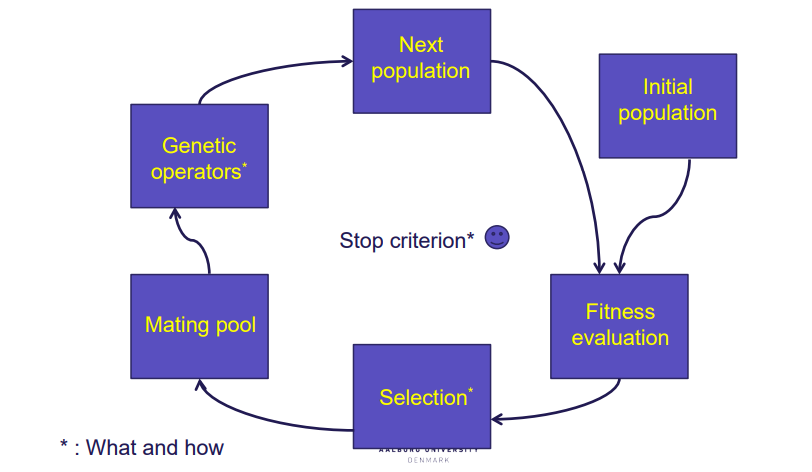
\includegraphics[width=\textwidth]{ga-cycle.png}
\end{figure}
\begin{figure}[!h]
\centering
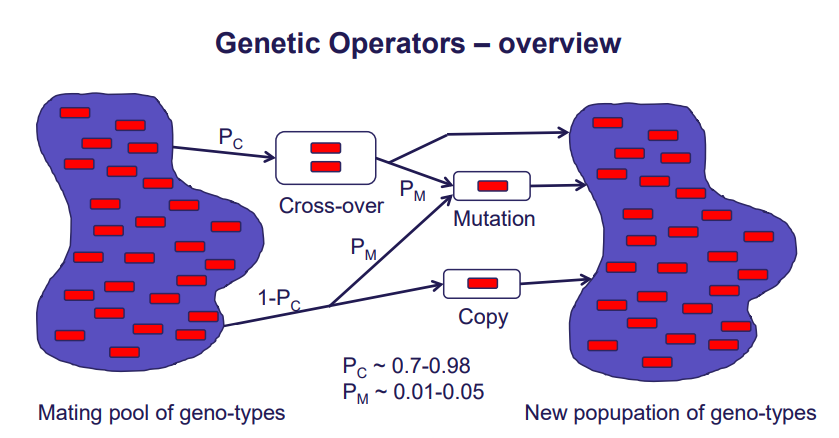
\includegraphics[width=\textwidth]{genetic_operators.png}
\end{figure}







\end{document}